% Author: Izaak Neutelings (May 2020)
\documentclass[border=3pt,tikz]{standalone}
\tikzset{>=latex} % for LaTeX arrow head
\usepackage{etoolbox} % ifthen
\usepackage{xcolor}
\usepackage{physics}
\usepackage{siunitx}

\colorlet{myblue}{blue!50!black}
\colorlet{mypurple}{blue!40!red!95!black}
\colorlet{mygreen}{green!70!black!60}
\colorlet{myyellow}{yellow!90!black!60}
\colorlet{myred}{red!80!black!60}
\pgfdeclareverticalshading{rainbow}{100bp}{
  color(0bp)=(red); color(25bp)=(red); color(35bp)=(yellow);
  color(45bp)=(green); color(55bp)=(cyan); color(65bp)=(blue);
  color(75bp)=(violet); color(100bp)=(violet)
}


\begin{document}


% SOUND DECIBEL SCALE
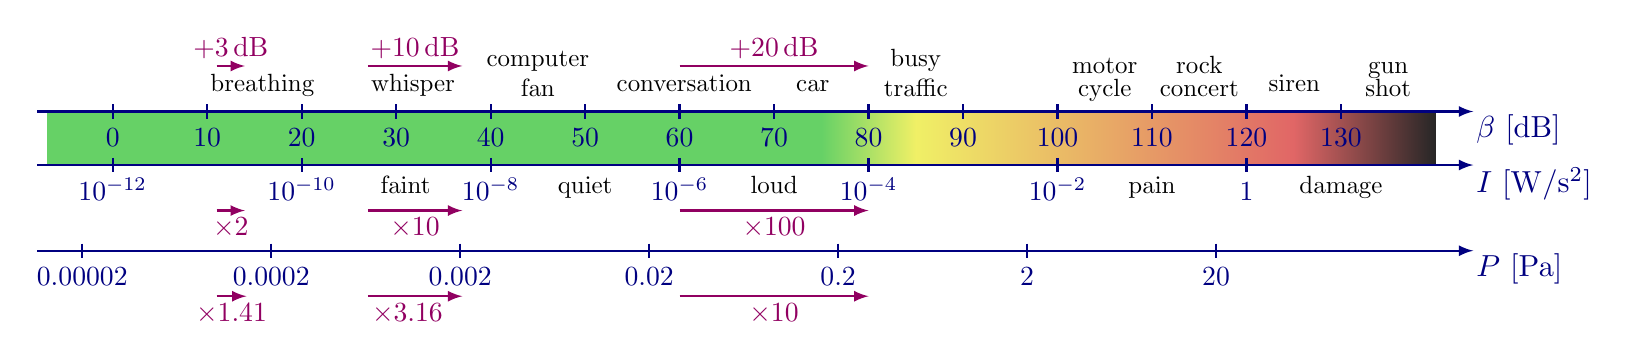
\begin{tikzpicture}[xscale=0.12]
  \def\h{0.68}
  
  \def\tick#1#2#3{\draw[thick,#2] (#1+.09) --++ (0,-.18) node[below=-2pt,scale=1] {\strut #3};}
  
  % MIDDLE
  \fill[mygreen] (-7,0) rectangle (80,\h);
  \fill[left color=mygreen,right color=myyellow]
    (75,0) rectangle (85,\h);
  \fill[left color=myyellow,right color=myred]
    (85,0) rectangle (125,\h);
  \fill[left color=myred,right color=black!85]
    (125,0) rectangle (140,\h);
  
  % DECIBEL
  \draw[->,thick,myblue] (-8,\h) -- (144,\h) node[below right=-3,scale=1.1] {$\beta$ [\si{dB}]};
  \foreach \x in {0,10,...,130}{
    \tick{\x,\h}{myblue}{$\x$}
  }
  \node[above right=-2,scale=0.9] at (10,1.15*\h) {\strut breathing};
  \node[above right=-2,scale=0.9] at (27,1.15*\h) {\strut whisper};
  \node[above=-4,scale=0.9,align=center]
    at (45,1.15*\h) {computer\\[0mm]\strut fan};
  \node[above right=-2,scale=0.9] at (53,1.15*\h) {\strut conversation};
  \node[above=-4,scale=0.9,align=center]
    at (85,1.15*\h) {busy\\[0mm]\strut traffic}; %vacuum cleaner
  \node[above right=-2,scale=0.9] at (72,1.15*\h) {\strut car};
  \node[above=-4,scale=0.9,align=center]
    at (105,1.15*\h) {motor\\[-1mm]\strut cycle};
  \node[above=-4,scale=0.9,align=center]
    at (115,1.15*\h) {rock\\[-1mm]\strut concert};
  \node[above right=-2,scale=0.9] at (122,1.15*\h) {\strut siren};
  \node[above=-4,scale=0.9,align=center]
    at (135,1.15*\h) {gun\\[-1mm]\strut shot};
  
  % ARROWS
  % +10 dB: 10^(10/20) = 3.1622776602
  % +20 dB: 10^(20/20) = 10
  \draw[->,thick,mypurple] (11, 1.85*\h) --++ (  3,0) node[midway,above=-1] {$+\SI{3}{dB}$};
  \draw[->,thick,mypurple] (27, 1.85*\h) --++ ( 10,0) node[midway,above=-1] {$+\SI{10}{dB}$};
  \draw[->,thick,mypurple] (60, 1.85*\h) --++ ( 20,0) node[midway,above=-1] {$+\SI{20}{dB}$};
  \draw[->,thick,mypurple] (11,-0.85*\h) --++ (  3,0) node[midway,below=-1] {$\times2$};
  \draw[->,thick,mypurple] (27,-0.85*\h) --++ ( 10,0) node[midway,below=-1] {$\times10$};
  \draw[->,thick,mypurple] (60,-0.85*\h) --++ ( 20,0) node[midway,below=-1] {$\times100$};
  \draw[->,thick,mypurple] (11,-2.45*\h) --++ (3.16,0) node[midway,below=-1] {$\times1.41$};
  \draw[->,thick,mypurple] (27,-2.45*\h) --++ (  10,0) node[pos=0.42,below=-1] {$\times3.16$};
  \draw[->,thick,mypurple] (60,-2.45*\h) --++ (  20,0) node[midway,below=-1] {$\times10$};
  
  % INTENSITY
  \draw[->,thick,myblue] (-8,0) -- (144,0) node[below right=-3,scale=1.1] {$I$ [\si{W/s^2}]};
  \foreach \x/\i in {0/-12,20/-10,40/-8,60/-6,80/-4,100/-2,120/0}{
    \ifnumcomp{\i}{<}{0}{
      \tick{\x,0}{myblue}{$10^{\i}$}
    }{
      \tick{\x,0}{myblue}{$1$}
    }
  }
  \node[below=-4,scale=0.9] at ( 31,-0.18*\h) {\strut faint};
  \node[below=-4,scale=0.9] at ( 50,-0.18*\h) {\strut quiet};
  \node[below=-4,scale=0.9] at ( 70,-0.18*\h) {\strut loud};
  \node[below=-4,scale=0.9] at (110,-0.18*\h) {\strut pain};
  \node[below=-4,scale=0.9] at (130,-0.18*\h) {\strut damage};
  
  % WATTS
  % I = P/(2*rho*v)
  % rho = 1.225 kg/m3 air
  % v = 343 m/s
  % 2*rho*v = 2*1.225*343 = 840.35 kg.s/m2
  % sqrt(2*1.225*343) = 28.9887909372
  % sqrt(2*1.225*343)*1e-6/(20e-6) = 1.4494395469
  % 10*log((2e-5)^2/(2*1.225*343)/1e-12) = -3.2240021308
  \draw[->,thick,myblue] (-8,-1.6*\h) -- (144,-1.6*\h) node[below right=-3,scale=1.1] {$P$ [Pa]};
  \foreach \x/\P in {0/0.00002,20/0.0002,40/0.002,60/0.02,80/0.2,100/2,120/20}{
    \tick{\x-3.22,-1.6*\h}{myblue}{$\P$}
  }
  
\end{tikzpicture}


\end{document}
